\subsection{Data and kernel (E1)}

\Cref{tab:data} summarizes the processed data. Bookkeeping violations are rare (about one PA in
two thousand, after excluding censored walk-off transitions). The kernel reproduces observed run
expectancy at the start of an inning (state 0) within \EoneStateZeroMaxDiff{} runs in every season
2023--2026 (e.g.\ $\mathrm{RE}(0)=\EoneREzero$ in 2026), and the visit-weighted mean absolute
difference over all 24 states is at most \EoneWeightedDiff{} (\cref{fig:re24}). The largest
differences (up to \EoneMaxDiff{} runs) occur in states with a runner on third and fewer than two
outs, where the model is \emph{below} the empirical value. Two observations show that this is a
selection effect rather than a kernel error: the expected runs of each individual transition out
of those states match the data closely, and the outcome mix observed in those states is markedly
more favourable to the offence than the league mix (in 2024, from first-and-third with no outs,
18.7\% singles and 19.8\% strikeouts versus 14.2\% and 22.6\% overall). Innings reach those states
disproportionately against weak pitching or with strong hitters at the plate, which a
league-average run-expectancy calculation cannot reflect. Game-level predictions (E3) use the
actual hitters and pitchers and are the relevant check.

\begin{figure}[t]\centering
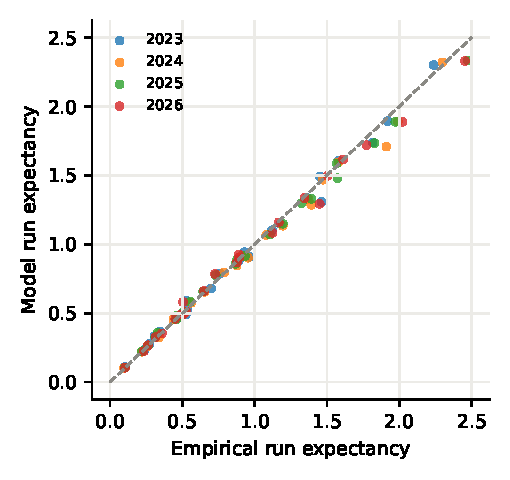
\includegraphics[width=0.48\textwidth]{figures/re24.pdf}\hfill
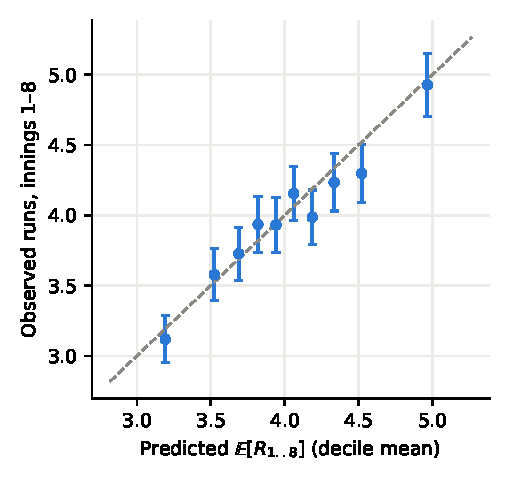
\includegraphics[width=0.48\textwidth]{figures/calibration.pdf}
\caption{Left: model versus empirical run expectancy for the 24 base-out states, 2023--2026 (E1).
Right: observed runs in innings 1--8 versus predicted expected runs, by decile of the prediction,
2025--2026 test seasons, with $\pm2$ standard errors (E3).}\label{fig:re24}\label{fig:calibration}
\end{figure}

\subsection{Plate-appearance model (E2)}

Tuning on 2024 selected prior-strength scales $\lambda_B=\EtwoBatterScale$,
$\lambda_P=\EtwoPitcherScale$ and half-life $H=\EtwoHalfLife$ days; the strength scales are
interior to the final grid, and $H=180$ days, evaluated in the first grid, was worse.
\Cref{tab:e2} reports the test seasons. Batter multipliers reduce log-loss relative to the league
model by about one hundredth of a nat per PA, and pitcher multipliers by a further 0.01; both
differences are large relative to their bootstrap intervals. Tuning the priors matters little
(about 0.001). The gradient-boosted model M3, using the same inputs, is better than M2 by 0.0008
nats in 2025 (interval excluding zero) and indistinguishable in 2026. Class-wise calibration of M2
is shown in \cref{fig:pacal}.

\begin{table}[t]\centering\small
\caption{Held-out log-loss (nats per PA) and difference from the full model with 95\% game-cluster bootstrap intervals. 2025: 186,562 PAs; 2026: 186,777 PAs.}\label{tab:e2}
\begin{tabular}{lcccc}\toprule
 & \multicolumn{2}{c}{2025} & \multicolumn{2}{c}{2026}\\
\cmidrule(lr){2-3}\cmidrule(lr){4-5}
Stage & Log-loss & $\Delta$ vs full & Log-loss & $\Delta$ vs full\\ \midrule
League rates & 1.7724 & $+$0.0278 [$+$0.0267, $+$0.0289] & 1.7735 & $+$0.0265 [$+$0.0255, $+$0.0276] \\
+ batter & 1.7547 & $+$0.0102 [$+$0.0095, $+$0.0109] & 1.7563 & $+$0.0093 [$+$0.0087, $+$0.0100] \\
+ pitcher (full model) & 1.7446 & --- & 1.7470 & --- \\
\bottomrule\end{tabular}\end{table}


\paragraph{Deviation from the pre-specified selection rule.} Our protocol selected the simplest
model not significantly worse than the best; strictly applied to 2025, it would select M3. We kept
M2 for the lineup analysis and report this as a deviation, for two reasons that we checked
rather than assumed. First, M2 provides the posterior distribution used for parameter uncertainty
(\cref{sec:uncertainty}), which M3 does not. Second, the choice does not change the decisions: on
\EtwocN{} random test team-games, the optimal order under M2 coincides with the M3 optimum in
\EtwocSame{} of the games, the M2 optimum loses on average \EtwocLoss{} runs per game when
evaluated under M3 (maximum \EtwocLossMax{}), the mean gains over the actual order are
\EtwocUpTwo{} (M2) and \EtwocUpThree{} (M3), and the correlation between the two models' values
over all 9! orders averages \EtwocCorr{}.

\paragraph{The original model.} On the window where its stored features exist (\EtwobWindow{},
\EtwobN{} PAs, which are out of sample for it), the predecessor system's 51-feature LightGBM has
log-loss \EtwobLegacyLL{} on the common seven-class taxonomy, against \EtwobMtwoLL{} for M2 and
\EtwobMzeroLL{} for the league model: M2 is better by \EtwobDiff{} nats per PA (95\% interval
\EtwobDiffLo{} to \EtwobDiffHi{}), despite the legacy features being recomputed daily rather than
every two weeks.

\begin{figure}[t]\centering
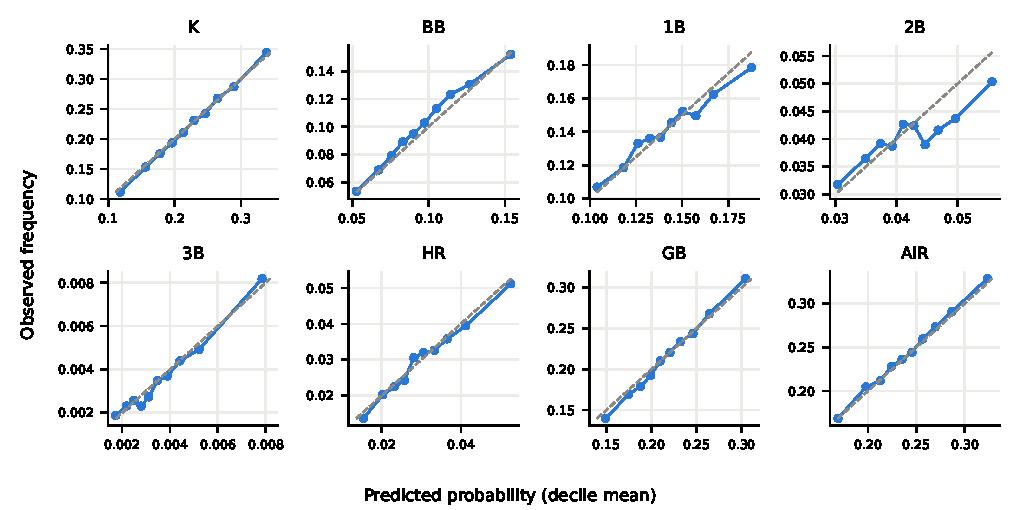
\includegraphics[width=\textwidth]{figures/pa_calibration.pdf}
\caption{Class-wise calibration of M2 on 2026 (deciles of the predicted probability).}\label{fig:pacal}
\end{figure}

\subsection{Run predictions at the game level (E3)}

Over \EthreeN{} test team-games, the mean prediction error (observed minus predicted runs in
innings 1--8) is \EthreeBias{} runs (95\% interval \EthreeBiasLo{} to \EthreeBiasHi{}), and the
calibration slope is \EthreeSlope{} (95\% interval \EthreeSlopeLo{} to \EthreeSlopeHi{}); neither
indicates miscalibration (\cref{fig:calibration}). The mean squared error is \EthreeMseModel{},
compared with \EthreeMseConst{} for the previous season's league mean and \EthreeMseTeam{} for
the team's mean over its previous 60 games. The correlation between predicted and observed runs
is only \EthreeCorr{}: almost all of the variance of a single game's runs is unpredictable before
the game. Randomized PIT values of the exact predicted run distributions on \EthreePitN{} random
team-games are close to uniform, and the central 80\% predictive interval covers
\EthreeCoverage{} of outcomes (\cref{fig:pit}); with integer-valued outcomes and inclusive interval
endpoints, coverage slightly above nominal is expected.

\begin{figure}[t]\centering
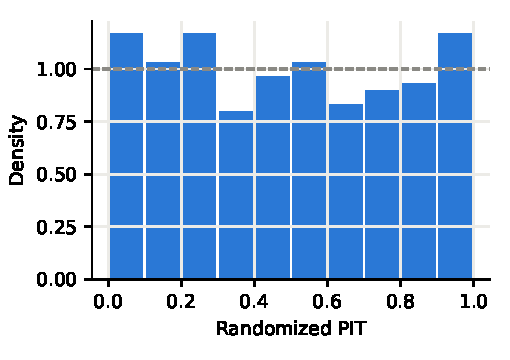
\includegraphics[width=0.48\textwidth]{figures/pit.pdf}
\caption{Randomized PIT histogram of observed runs in innings 1--8 (E3).}\label{fig:pit}
\end{figure}

\subsection{Search methods (E4a)}

\Cref{tab:e4a} compares the search methods with the exhaustive optimum. Exhaustive search takes
\EfouraExhaustiveSeconds{}~s per instance on one machine (all 362{,}880 orders). Local search from
ten random starts found the optimum in every instance tested, and simulated annealing and the
genetic algorithm with exact fitness came close, so for this problem size the choice among
competent search methods is unimportant once the objective is exact; exhaustive search is
preferred because it provides the certificate of \cref{cor:cert}. The heuristic guideline of
\citet{tango2007} recovers about half of the gap between the actual order and the optimum.

The genetic algorithm with Monte Carlo fitness, as in the predecessor system, performs worse
than the managers' own orders (mean gap \EfouraNoisyGap{} runs), and its reported value of the
chosen order exceeds the order's exact value by \EfouraCurse{} runs on average
(\EfouraNoisyN{} instances): the optimizer's curse is an order of magnitude larger than the
effect being optimized. With 4{,}000 simulated games, the standard error of one fitness evaluation
is about $3/\sqrt{4000}\approx0.05$ runs, larger than the differences among good orders.

\begin{table}[t]\centering\small
\caption{Search methods on 200 random 2026 regular-season team-games. Gap: exact $V(\pi^\star)-V(\hat\pi)$ in runs per game; Optimal: share of instances where the exact optimum was returned. $^\dagger$On 30 of them.}\label{tab:e4a}
\begin{tabular}{lrrrr}\toprule
Method & Mean gap & Max gap & Optimal & Evaluations\\ \midrule
Exhaustive search (exact) & 0.0000 & 0.0000 & 100\% & 362,880 \\
2-swap local search, 10 starts & 0.0000 & 0.0000 & 100\% & 1,933 \\
Simulated annealing & 0.0000 & 0.0021 & 94\% & 1,707 \\
Genetic algorithm, exact fitness & 0.0001 & 0.0034 & 82\% & 523 \\
2-swap local search from actual order & 0.0004 & 0.0091 & 68\% & 203 \\
\citeauthor{tango2007} guideline & 0.0092 & 0.0251 & 0\% & 0 \\
Sort by run value & 0.0092 & 0.0306 & 1\% & 0 \\
Sort by on-base probability & 0.0110 & 0.0341 & 0\% & 0 \\
Order actually used & 0.0186 & 0.0641 & 0\% & 0 \\
Original GA, Monte Carlo fitness$^\dagger$ & 0.0223 & 0.0526 & 0\% & 1,710 \\
\bottomrule\end{tabular}\end{table}


\subsection{How far are real orders from the optimum? (E4b)}

Across \EfourbN{} team-games of 2025--2026, the model-optimal order exceeds the order actually used
by \EfourbUpliftMean{} expected runs per game on average (median \EfourbUpliftMedian{}, 90th
percentile \EfourbUpliftQninety{}, maximum \EfourbUpliftMax{}), or \EfourbUpliftSeason{} runs per
162 games if the gap persisted every day (\cref{fig:uplift}). The best and the worst of all 9!
orders differ by only \EfourbSpread{} runs per game on average, and the optimum exceeds the average
of a uniformly random order by \EfourbOptVsRandom{}. Orders actually used rank, on median, above
\EfourbPctMedian{} of all possible orders, and \EfourbShareAboveNinety{} of them are above the 90th
percentile. In this model, therefore, managers' orders are close to optimal and the room for
improvement is a few runs per season, in line with the classical literature
\cite{freeze1974,tango2007}.

\begin{figure}[t]\centering
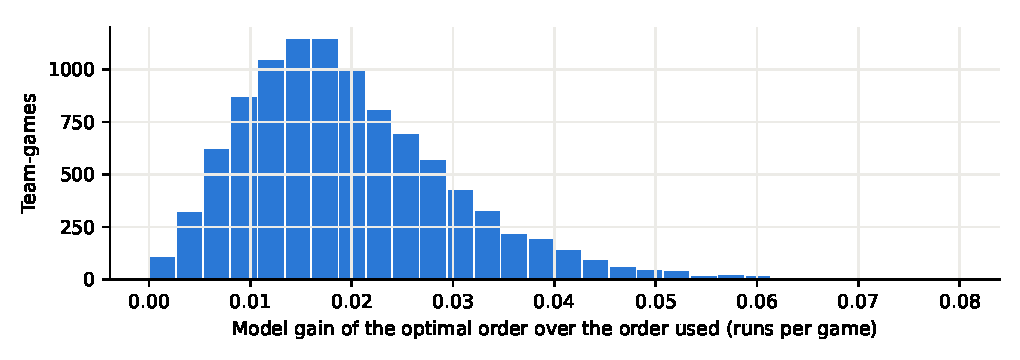
\includegraphics[width=\textwidth]{figures/uplift_hist.pdf}
\caption{Model gain of the optimal order over the order actually used, 2025--2026 (E4b).}\label{fig:uplift}
\end{figure}

\subsection{Parameter uncertainty}\label{sec:uncertainty}

In \EfourcN{} random 2026 team-games with \EfourcDraws{} posterior draws each (E4c), the point-
estimate optimal order is better than the actual order in \EfourcPBetter{} of draws on average,
but the 90\% posterior interval of the gain excludes zero in only \EfourcExcl{} of games, and its
mean width (\EfourcWidth{} runs) exceeds the typical gain. The exact optimal order changes in almost
every draw (it is unchanged in \EfourcSame{} of draws): many orders are nearly tied, and the data
cannot single out one of them. What the data do support is a statement about a set of good orders
(those that move the best hitters up), not about a unique best order.

\subsection{The 2026 World Series, Game 5 (E5)}

Milwaukee won 4--1 at Tropicana Field. Facing Drew Rasmussen and the Tampa Bay bullpen, the order
Milwaukee used has model value \RefActualAway{} expected runs over nine innings; the optimal order
\RefOptimalAway{} (gain \RefUpliftAway{}, 90\% interval \RefLoAway{} to \RefHiAway{}, optimal
better in \RefPBetterAway{} of \RefDraws{} posterior draws). The order used ranks above
\RefPctAway{} of all orders. For Tampa Bay, facing Jacob Misiorowski and the Milwaukee bullpen, the
values are \RefActualHome{} and \RefOptimalHome{} (gain \RefUpliftHome{}, interval \RefLoHome{} to
\RefHiHome{}, better in \RefPBetterHome{} of draws; rank \RefPctHome{}). The observed scores
(\RefObservedAway{} and \RefObservedHome{} runs) are single draws from predictive distributions
with a standard deviation of about three runs and carry essentially no information about the
merit of either order (\cref{rem:identification}). \Cref{tab:ref} lists the orders.

\begin{table}[t]\centering\small
\caption{2026 World Series Game 5: starting orders used and model-optimal orders (information before 2026-10-28).}\label{tab:ref}
\begin{tabular}{rllll}\toprule
 & \multicolumn{2}{c}{Milwaukee Brewers} & \multicolumn{2}{c}{Tampa Bay Rays}\\
\cmidrule(lr){2-3}\cmidrule(lr){4-5}
Slot & Used & Optimal & Used & Optimal\\ \midrule
1 & Jackson Chourio & Brice Turang & Yandy Díaz & Liam Hicks \\
2 & Jake Bauers & Jake Bauers & Jonathan Aranda & Jonathan Aranda \\
3 & Christian Yelich & William Contreras & Junior Caminero & Junior Caminero \\
4 & William Contreras & Jackson Chourio & Liam Hicks & Yandy Díaz \\
5 & Brice Turang & Cooper Pratt & Jonny DeLuca & Chandler Simpson \\
6 & Sal Frelick & Christian Yelich & Chandler Simpson & Ryan Vilade \\
7 & Cooper Pratt & Garrett Mitchell & Ben Williamson & Jonny DeLuca \\
8 & Garrett Mitchell & Sal Frelick & Ryan Vilade & Ben Williamson \\
9 & David Hamilton & David Hamilton & Taylor Walls & Taylor Walls \\
\bottomrule\end{tabular}\end{table}

